%!TEX root = paper.tex
%%%%%%%%%%%%%%%%%%%%%%%%%%%%%%%%%%%%%%%%%%%%%%%%%%%%%%%%%%%%%%%%%%%%%%%%%%%%%%%%
\section{Overview and Background}
\label{sec:background}

Before diving into the promised end-to-end lag model, some terms and concepts need to be introduced first.


\subsection{Game Types}
%TODO: needs a better word than types, more like architectures. Feedback welcome
Describe different types of games, i.e. local games, client-server games, streamed games.

% TODO: We could use one figure with three subfigures which shows the (ever increasing)
%       number of components 

\paragraph*{Local Games}

\begin{figure}
  \centering
  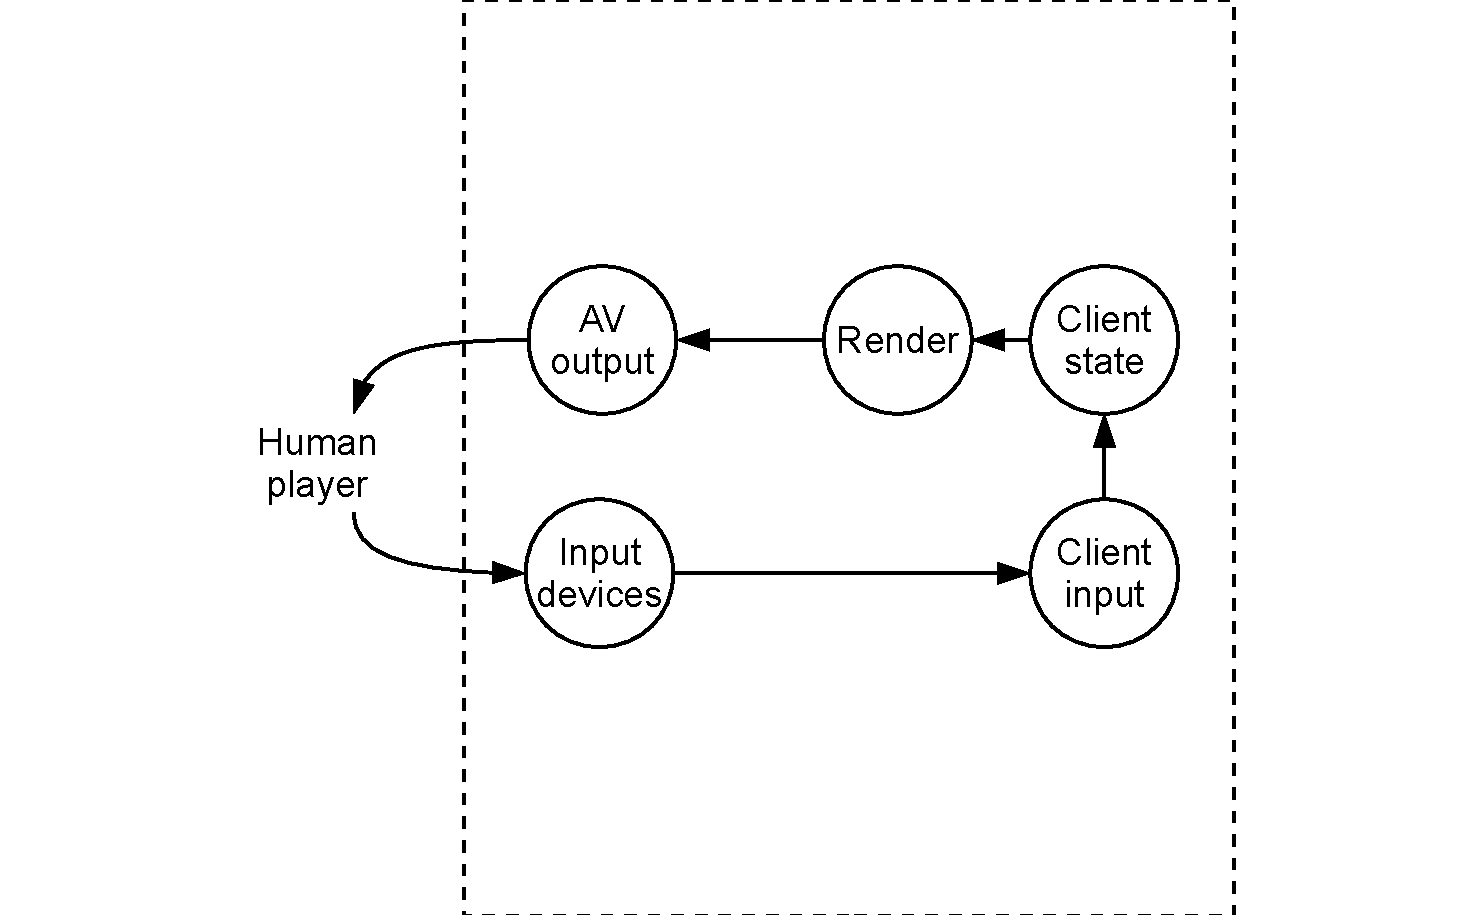
\includegraphics[width=0.8\columnwidth]{../models/component_interaction-local.pdf}
  \caption{Interaction of TODO.}
  \label{fig:component-model-local}
\end{figure}

\paragraph*{Client-Server Games}

\begin{figure}
  \centering
  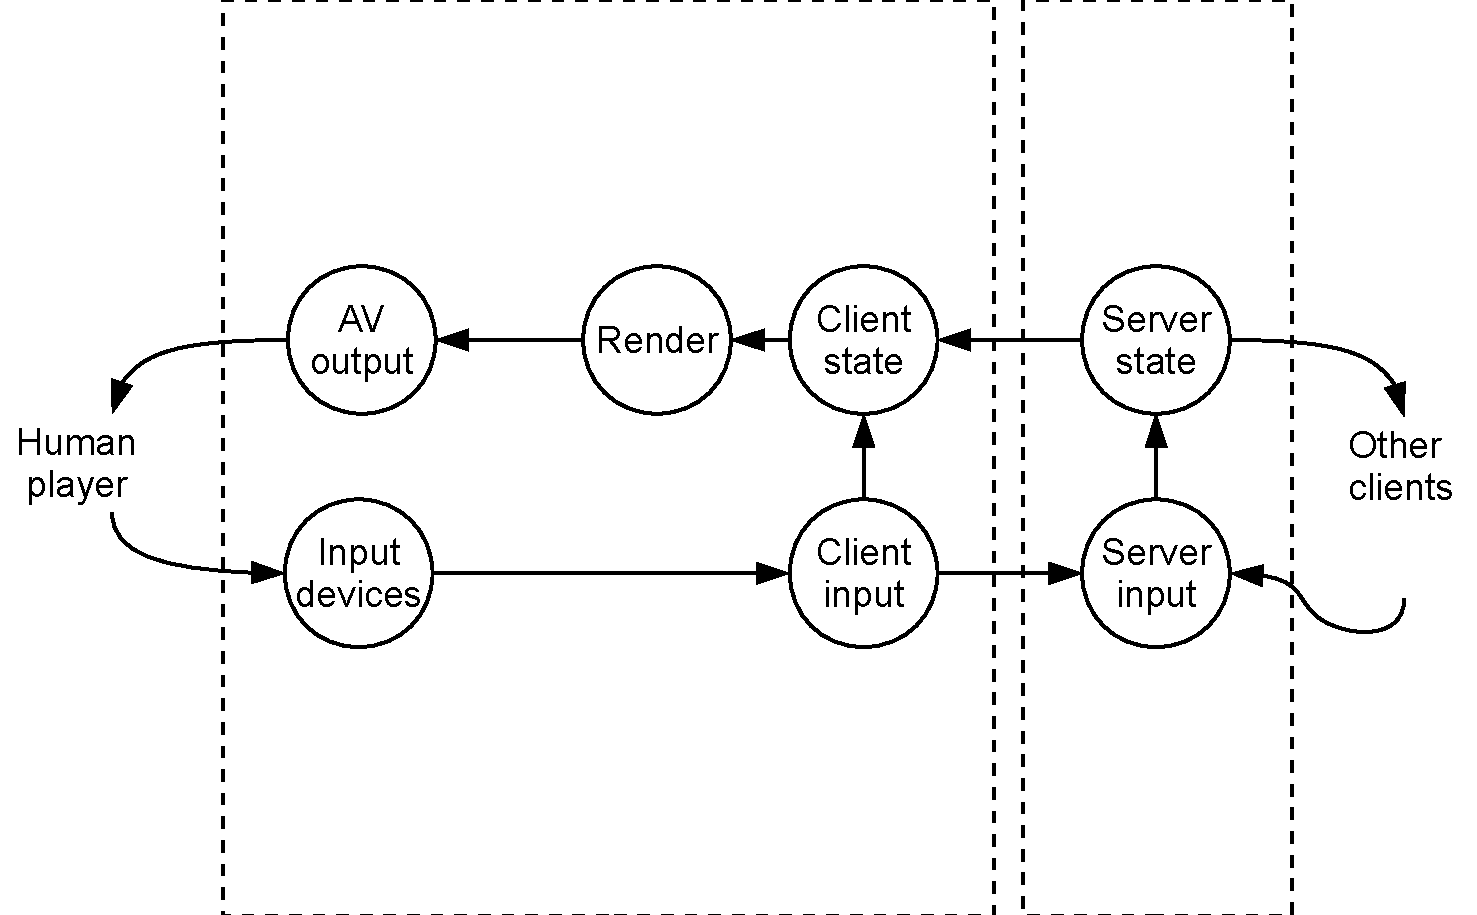
\includegraphics[width=0.8\columnwidth]{../models/component_interaction-online.pdf}
  \caption{Interaction of TODO.}
  \label{fig:component-model-online}
\end{figure}

\paragraph*{Streaming Games}

\begin{figure}
  \centering
  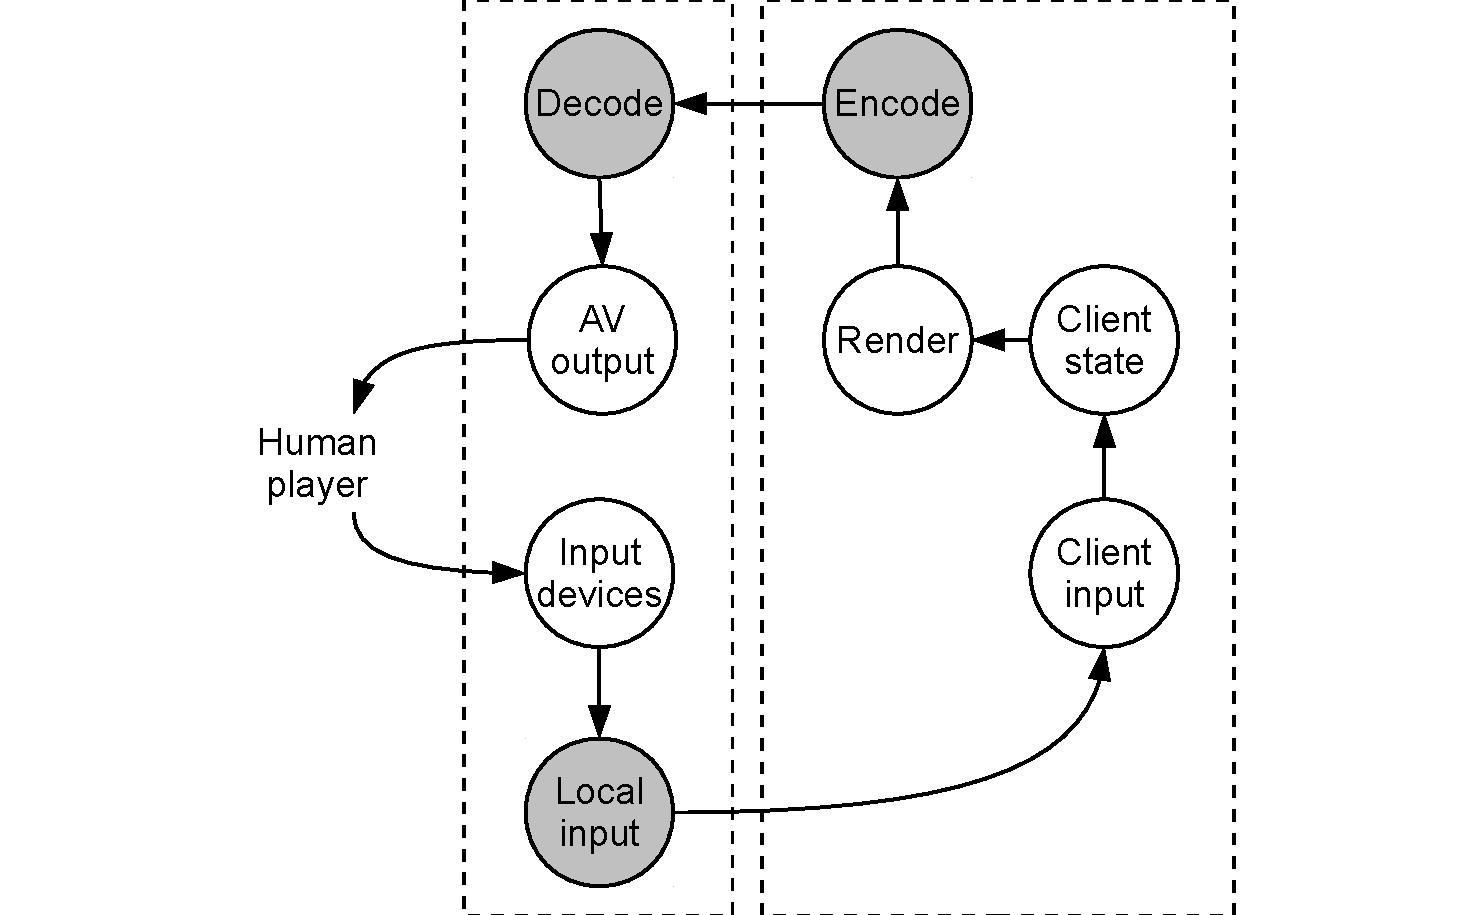
\includegraphics[width=0.8\columnwidth]{../models/component_interaction-cloud.pdf}
  \caption{Interaction of TODO.}
  \label{fig:component-model-cloud}
\end{figure}

\begin{figure}
  \centering
  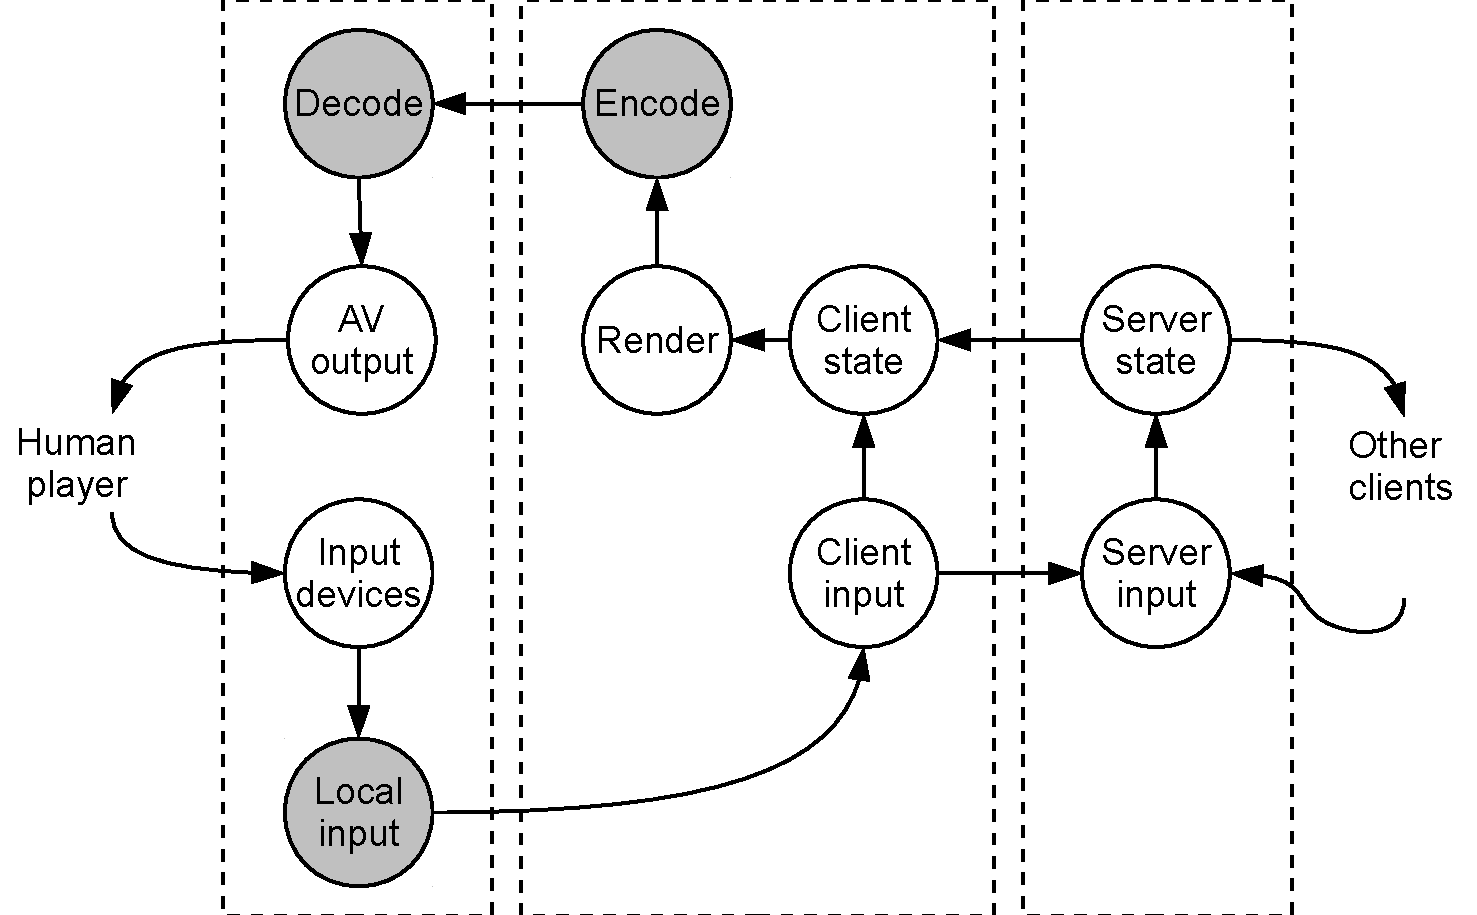
\includegraphics[width=0.8\columnwidth]{../models/component_interaction-online+cloud.pdf}
  \caption{Interaction of TODO.}
  \label{fig:component-model-online+cloud}
\end{figure}

At the end of this subsection, the reader should understand which (technological) components make up the different types of games.

\subsection{Big Picture}

This subsection adds the player to the architectures introduced above, highlights potential QoS and QoE (or discusses why some chosing a particular QoE metric is not useful) metrics to study.

% \begin{figure}
%   \centering
%   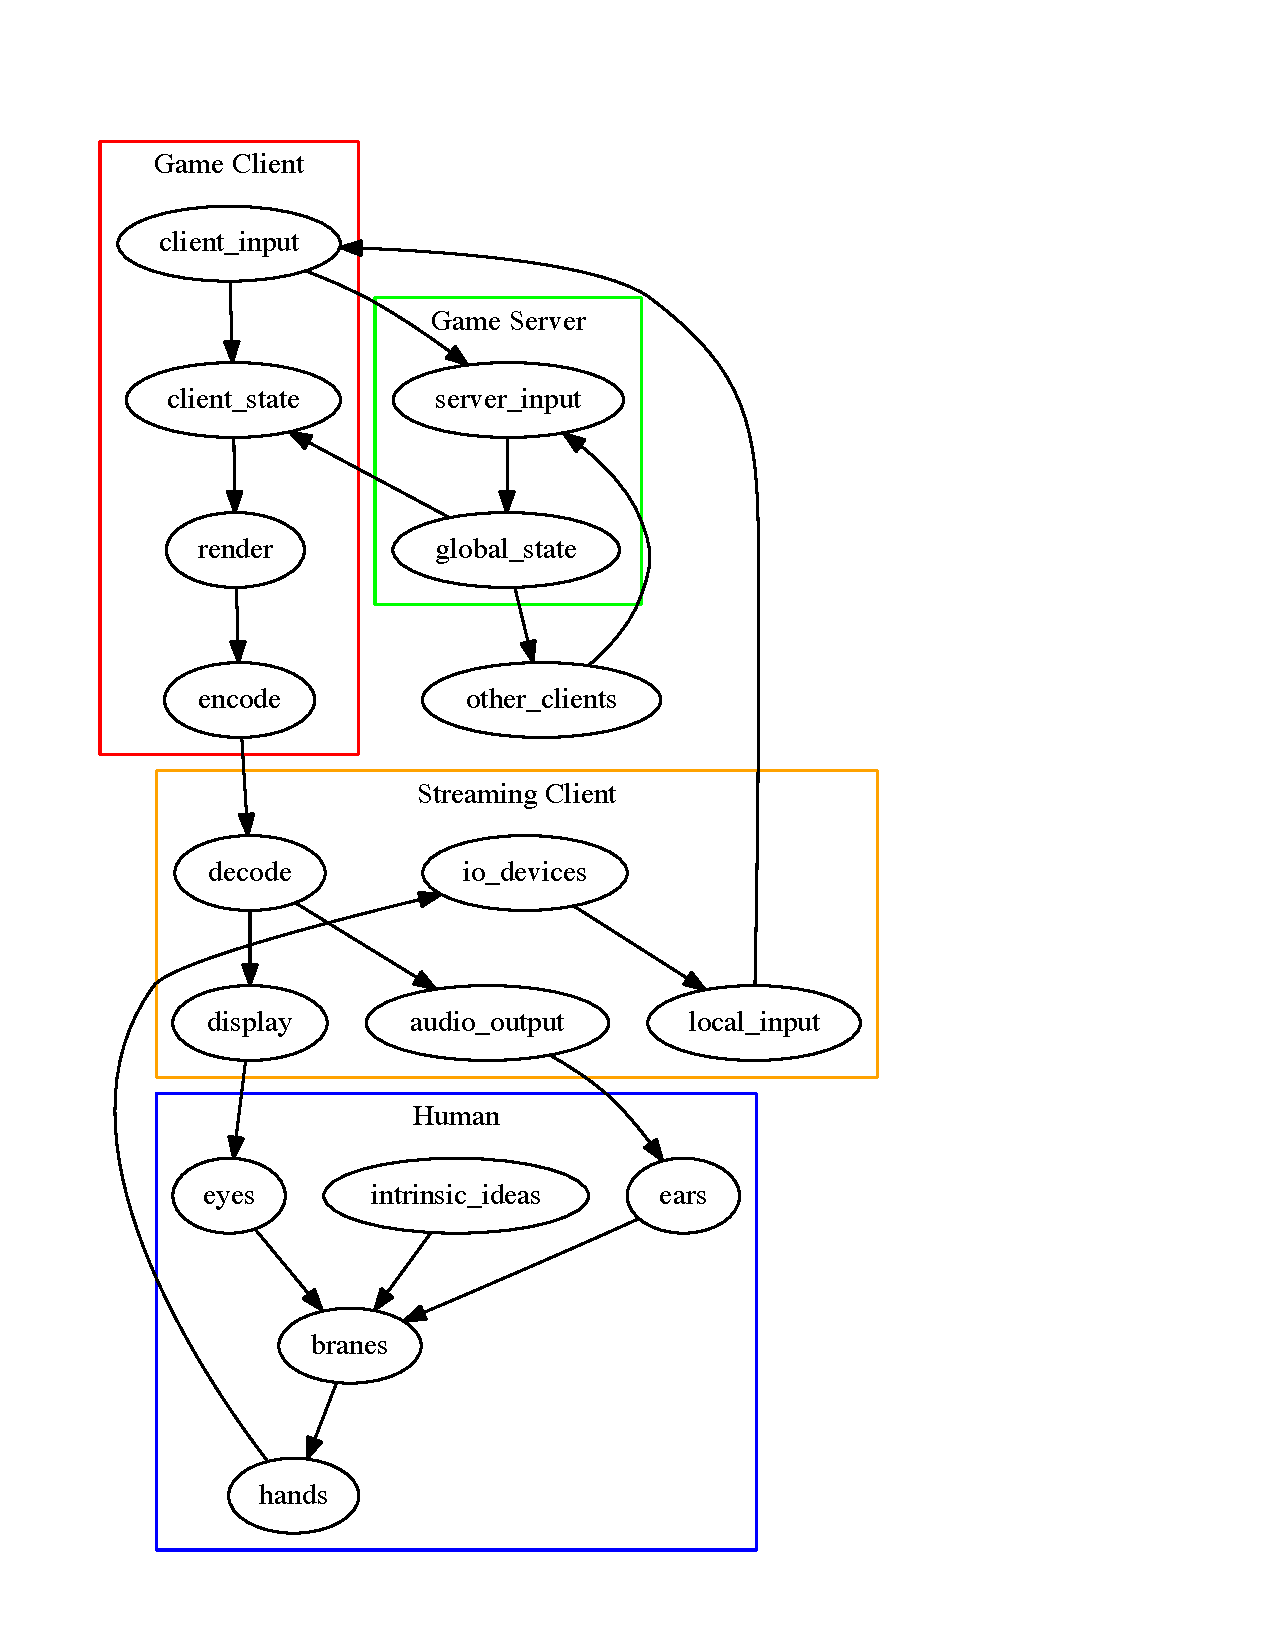
\includegraphics[width=1.0\columnwidth]{../models/cycle.pdf}
%   \caption{Interaction of TODO.}
%   \label{fig:component-model}
% \end{figure}

At the end of this section, the reader should agree that end to end latency is a sensible starting point to study video game qos.


%%%%%%%%%%%%%%%%%%%%%%%%%%%%%%%%%%%%%%%%%%%%%%%%%%%%%%%%%%%%%%%%%%%%%%%%%%%%%%%%
\subsection{Measurement Approaches}
\label{sec:measurementapproaches}

With these metrics, test parameters, and categorizations in mind, one can now attempt to conduct the actual measurements of which there are three distinct methods each situated at a unique vantage point as depicted in Fig.~\ref{fig:measurement-methods}.

\begin{figure}[!t]
    \centering
    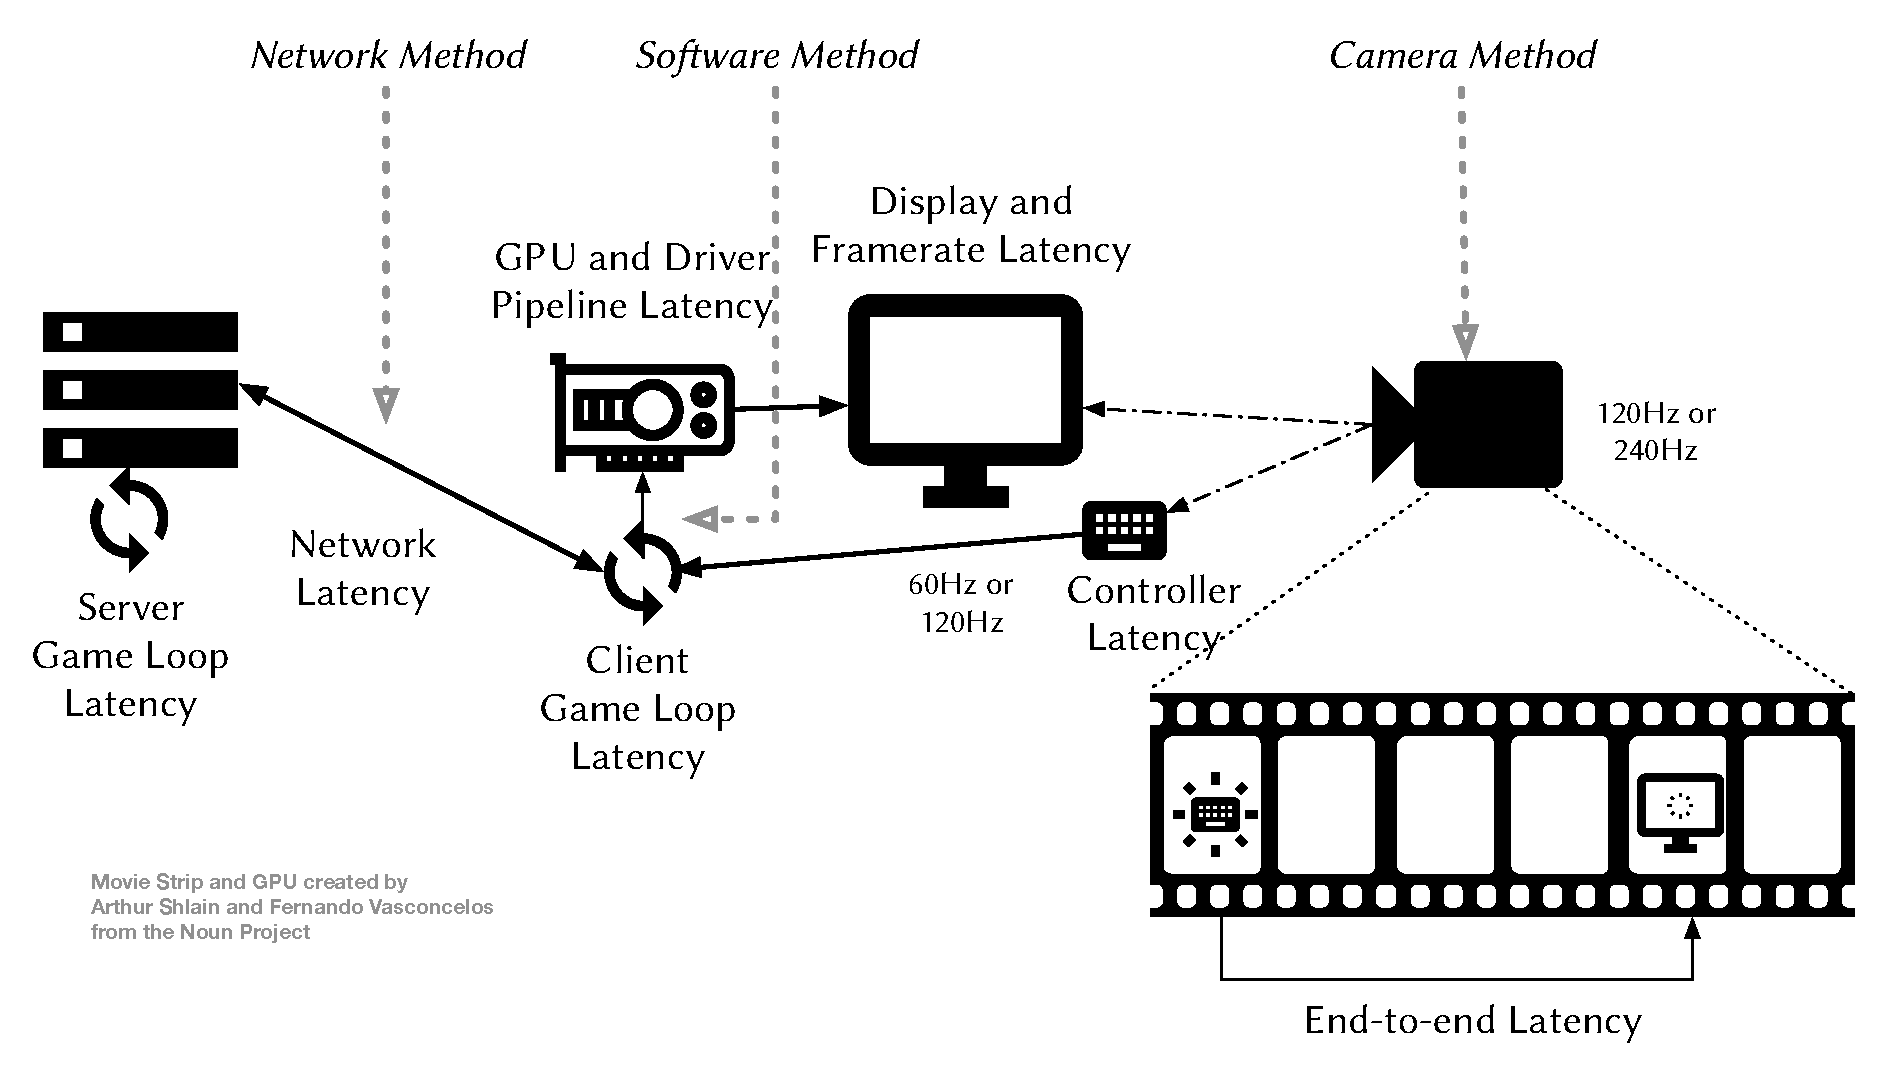
\includegraphics[width=1.0\columnwidth]{../models/e2e-lag.pdf}
    \caption{Location of the three measurement approaches to capture end-to-end latency inside a usual online video game lag chain.}
\label{fig:measurement-methods}
\end{figure}



